\Huge\textbf{Capitolo 6: \\Citoscheletro}

\vspace{1cm}
\small
Il citoscheletro è una struttura cellulare composta da microtubuli (MT), filamenti intermedi (FI) e microfilamenti (MF). Hanno funzioni, dimensioni e composizioni molecolari differenti.

\section{Microtubuli}
    I MT hanno un diametro di circa 25 nm e sono l'"impalcatura" per il traffico intracellulare. Sono presenti in ogni tipologia cellulare e hanno struttura sempre uguale a se stessa, ma assumono funzioni differenziate.
    \subsection{Struttura e conformazioni}
        Un MT è un cilindro cavo composto da 13 protofilamenti lineari con simmetria radiale. I protofilamenti sono eterodimeri composti da sequenze alternate di $\alpha$tubulina ($\alpha$T) e $\beta$tubulina ($\beta$T). $\alpha$T si associa sempre a GTP (funzione di cofattore) mentre $\beta$T si può associate a GTP o GDP (funzione di cofattore) e catalizza eventualmente l'idrolisi da GTP a GDP.
        \begin{figure}[h]
            \centering
            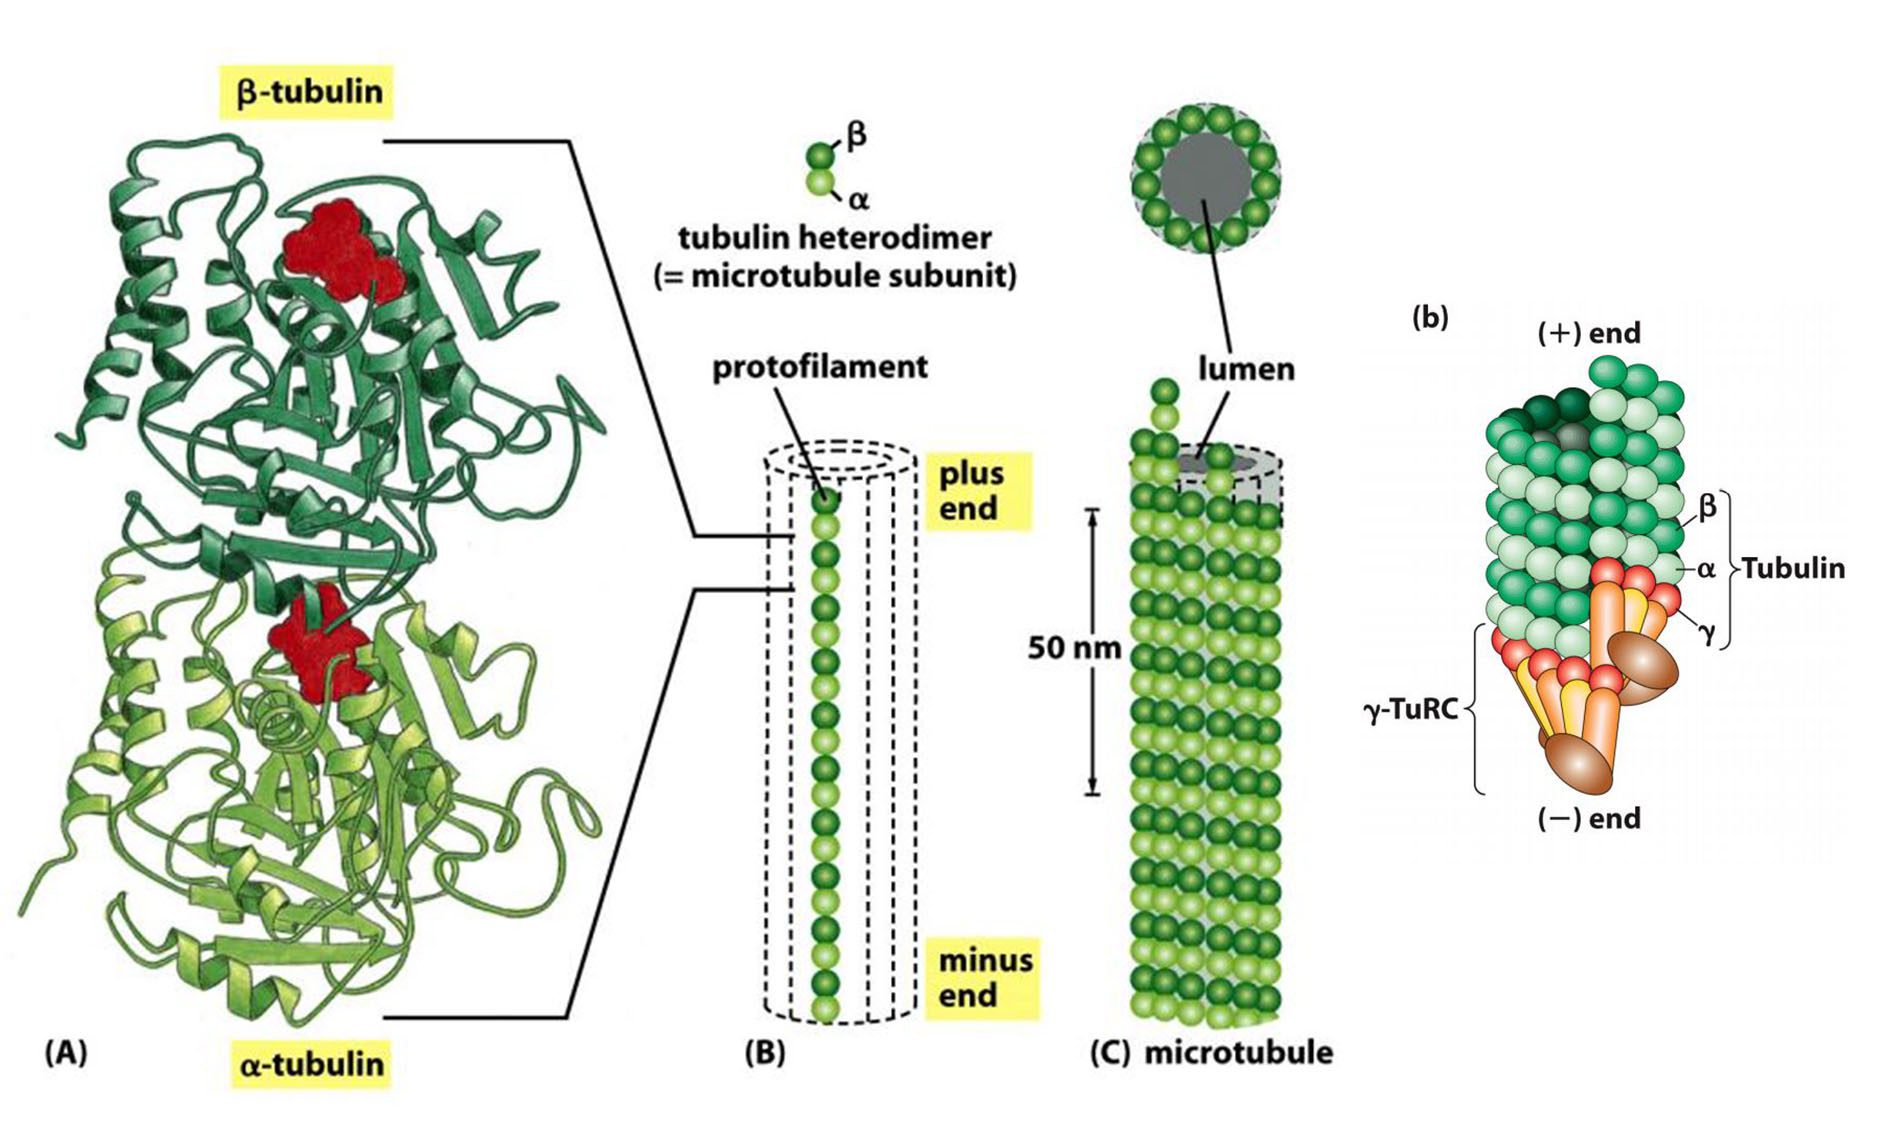
\includegraphics[width=0.8\textwidth]{images/MT.JPG}
            \caption{\small struttura di un microtubulo}
            \label{fig:mesh1}
        \end{figure}
        I protofilameti sono eterodimeri orientati ($\alpha$T , negativa - $\beta$T, positiva) quindi intrinsecamente polari. I MT sono composti da 13 protofilamenti per la formazione di un cilindro cavo (la polarità del MT corrisponde alla polarità del protofilamento, i fasci sono paralleli e hanno la stessa polarità). L'andamento elicoidale fa sì che si verifichi una discontinuità chiamata seam visibile come stacco del pattern.    \\
        I MT possono assumere più strutture:
        \begin{itemize}
            \item singola: solamente un tubulo di 13 protofilamenti
            \item doppiette: un tubulo da 13 filamenti e uno da 10 
            \item triplette: un tubulo da 13 e due da 10
        \end{itemize}
        L'estremità negativa del MT è "incappucciata" a un cap chiamato $\gamma$TURC (\textit{tubulin ring complex}), un complesso formato da 14 molecole di $\gamma$ tubulina ($\gamma$T). L'ultima $\alpha$T è associata ad una $\alpha$T che lega GTP.
        Questo protegge l'estremità negativa e favorisce associazioni con altre proteine che predispongono alla nucleazione.
        \subsubsection{MTOC}
            I MT possono assumere conformazioni spaziali molto diverse, sempre polari con l'estremità negativa sempre associata ad un MTOC. (\textit{microtubule-organizing center}). In ogni cellula è sempre presente almeno un MTOC. Esempi di MTOC sono il centrosoma e il corpo basale di un cilio.\\
            Gli MTOC organizzano la conformazione spaziale della cellula e degli organelli. La densità dei MT aumenta in prossimità di un MTOC.\\
            
                \textbf{Centrosoma}\\
                Il centrosoma è il principale MTOC e al contempo un organello proteico senza membrana circondato da PCM (\textit{peri centriolar material}) contenente $\gamma$TURC. Ciascun centrosoma è composto da due centrioli disposti perpendicolarmente.\\
                Il centrosoma è composto di due centrioli così strutturati:
                \begin{itemize}
                    \item all'estremità basale sono presenti triplette di MT
                    \item all'estremità distale sono presenti doppiette di MT
                \end{itemize}
                Sono sempre composti di 9 triplette di MT equidistanti tra loro. Uno dei due centrioli è più vecchio e si dice \textit{madre} ed è morfologicamente diverso dal secondo. 
                Il centriolo madre ha nelle porzioni distale e sub-distale degli appendici. Il centriolo figlio non porta appendici ma presenta un \textit{cartwheel} nella porzione basale e ogni raggio della ruota lega una tripletta di MT. Il cartweel è una struttura transitoria che concorre alla formazione del centriolo (quindi utile alla fase iniziare della sintesi).\\
                Non è noto perchè sia necessario un organello così complesso per legare la $\gamma$T delle estremità negative dei MT.\\
                Le cellule vegetali non presentano centrioli, ma esistono altre forme di MTOC.\\
                Normalmente una cellula presenta un unico centrosoma. In fase di duplicazione viene anche esso duplicato ed è funzionale alla separazione della cellula, alla citochinesi e alla cariochinesi.
                \begin{figure}[h]
                    \centering
                    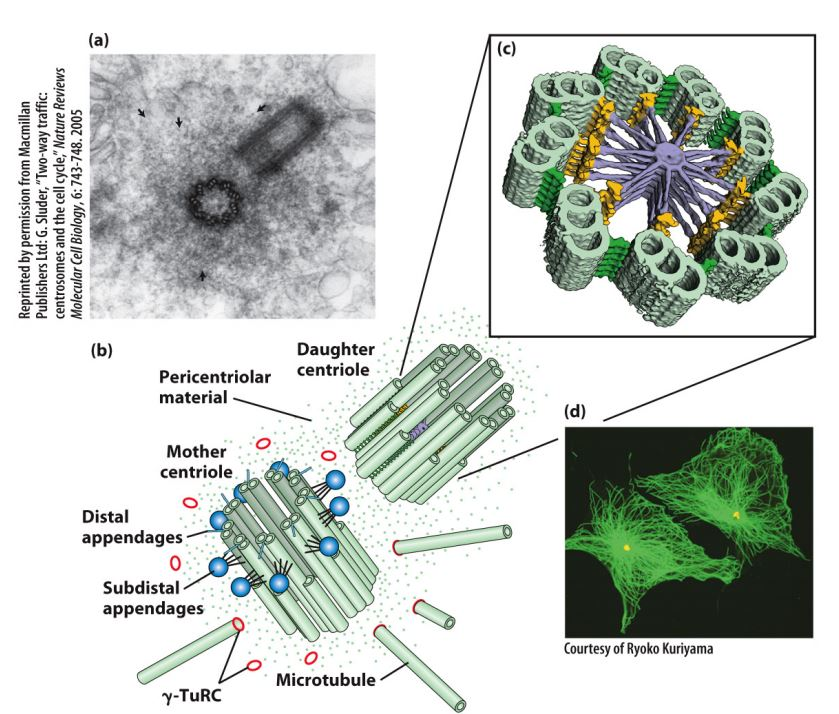
\includegraphics[width=0.5\textwidth]{images/centrosoma.JPG}
                    \caption{\small struttura di un centrosoma} 
                    \label{fig:mesh1}
                \end{figure}\\
                Il centrosoma assume ruoli differenti a seconda della fase cellulare:
                \begin{enumerate}
                    \item in fase di duplicazione forma organizza il fuso mitotico
                    \item può formare il corpuscolo basale per il cilio primario
                \end{enumerate}
                Il centriolo madre presenta gli appendici distali e sub-distali necessari per diventare basal body e nucleare il cilio.
        
    \subsection{Comportamento nella cellula}
        \subsubsection{Instabilità dinamica dei MT}
            Tra le estremità positive e negative dei MT affiora un'asimmetria: l'estremità positiva infatti accresce più velocemente di quella negativa. Studi in vitro suggeriscono che dopo una certa soglia, il MT depolimerizza (in base alla torbidità).\\
            In vitro, i dimeri di tubulina si associano in due direzioni. I legami longitudinali sono per lo più stabili, mentre quelli laterali soffrono grave instabilità nel momento in cui avviene una curvatura del MT dovuta alla presenza di GDP (se la curvatura è troppo pronunciata si verifica una catastrofe). Esistono farmaci che rendono le catastrofi più frequenti con il fine di danneggiare un tessuto tumorale.\\
            Si nota inoltre che fornendo i dimeri di tubulina, essi si associano spontaneamente nella formazione di un MT, sempre con la stessa organizzazione spaziale.\\
            
            \textbf{Catastrove}\\
                Si osserva in vitro una ritmica crescita e decrescita del MT, le seconde dovute alle cosiddette \textit{catastrofi}, durante le quali la velocità di decrescita supera quella della crescita.
                All'interno di una cellula succede lo stesso fenomeno, per ogni MT gli eventi sono asincroni e indipendenti.
                Il MT si associa stabilmente utilizzando GTP sia per $\beta$T che per $\alpha$T. Qualora il GTP associato alla $\beta$T venga idrolizzato, avviene un lieve cambio conformazionale che tende a incurvare il protofilamento. Questo evento favorisce la depolimerizzazione, quindi avviene una catastrofe.\\
                
            \textbf{Rescue}\\
                Alle catastrofi si alternano fasi di \textit{rescue}, durante le quali il GDP viene sostituito da GTP (processo endoergonico) per la costruzione di MT stabili.\\
            
            L'alternare di catastrofi e rescue definiscono l'instabilità dinamica intrinseca dei MT.
            \begin{figure}[h]
                    \centering
                    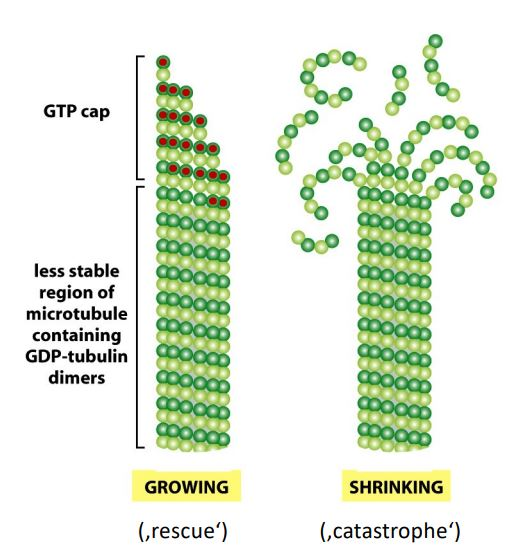
\includegraphics[width=0.5\textwidth]{images/rescue_catastrofe.JPG}
                    \caption{\small schema degli eventi di catastrofi e rescue}
                    \label{fig:mesh1}
            \end{figure}
            Quando viene idrolizzato GTP a GDP, non avviene una catastrofe immediatamente, bensì si crea una tensione del MT che viene sfruttata dalla cellula per muovere componenti cellulari o cercare altre componenti (ad esempio, esistono delle proteine che si associano specificamente all'estremità positiva in fase di depolimerizzazione per essere trascinate verso l'estremità negativa).\\
            Inoltre la stessa crescita e decrescita dinamica è sfruttata per "cercare" componenti, infatti la posizione centrale dei centrosomi e la possibilità di crescita e decrescita delle sue estremità positive, fanno sì che (anche stocasticamente) queste vengano in contatto con organelli o generalmente componenti cellulari (comprese proteine della membrana). Quindi hanno anche il compito di posizionare gli organelli.
                
        \subsubsection{Treadmilling}
            Il MT in vitro tende a polimerizzare all'estremità positiva mentre all'estremità negativa si nota una depolimerizzazione. Questo avviene meno frequentemente nelle condizioni normali della cellula perchè è presente all'estremità negativa $\gamma$TURC che protegge l'estremità.\\
            Il processo di depolimerizzazione all'estremità negativa e polimerizzazione a quella positiva favorisce una certa dinamicità, lo "scorrimento" del filamento si chiama appunto \textit{treadmilling}.
            
        \subsubsection{MAPS}
            Le MAPS (\textit{microtubule associated proteins}) modificano il comportamento dei MT.\\
            
            \textbf{TAU}\\
                TAU interagisce con i dimeri di tubulina (con domini specifici) elettrostaticamente per ne determina la distanza reciproca in base alla lunghezza di domini che protrudono dalle TAU stesse (lunghezza del dominio di TAU è inferiore a MAP2, ad esempio).\\
                
            \textbf{EB1}\\
                EB1 (end-binding protein) si lega alle estremità positive (in particolare il GTP cap). Tipicamente è associata ad altre proteine che sfruttano EB1 per essere trasportate (grazie l'instabilità dinamica).\\
                
            \textbf{Chinesina 13 (CHI13)}\\
                Altera il comportamento dei MT catalizzando l'energia per dissolvere il MT a livello del dimero (quindi promuove una catastrofe).\\
                
            \textbf{Stathmin}\\
                Hanno una conformazione a U con affinità per gli eterodimeri di $\alpha$T e $\beta$T. Nel momento in cui l'estremità positiva sia incurvata ne accentuano questa caratteristica.
        
    \subsection{Motor proteins}
        Le \textit{motor proteins} sono le proteine che sono associate al movimento di molecole o complessi maggiori lungo i MT.
        
        \subsubsection{Esperimenti}
            Marcando degli AA con radioattività, si nota come la proteina costruita con questo AA venga trasportata lungo i MT in verso sia anterogrado che retrogrado. Si nota inoltre che la velocità del trasporto è più alta rispetto al semplice trasporto in soluzione. Si deduce che ci sono delle componenti che si occupano del movimento di queste molecole (ovvero le motor proteins).\\
            Utilizzando l'assone gigante del calamaro, è possibile estrarre fasci di MT ed è possibile notare che le vescicole viaggiano lungo questo canale in senso anterogrado e retrogrado.
        
        \subsubsection{Chinesine}
            Sono una famiglia di motor proteins che si muovono per lo più dall'estremità negativa a quella positiva (tranne rare eccezioni), quindi in senso anterogrado. La prima scoperta è stata isolata dall'assone gigante del calamaro, ovvero CHI1.\\
            
            \textbf{Struttura} \\
                Le chinesine sono composte da due catene pesanti (stelo), due catene leggere, due teste e due code. \\
                Sulle teste è presente un nucleoside di-fosfato. Sono proprio le teste che interagiscono con il MT per "camminare".\\
                Trasportano un cargo tramite dei legami con le catene leggere attraverso in recettore per la CHI presente sul cargo.\\
            
            \textbf{Classificazione}\\
                Le chinesine (CHI) sono divise in 14 classi differenti, codificare da 45 geni diversi (nel genoma umano). La struttura della testa resta per lo più simile tra le classi, altri domini presentano un'elevata eterogeneità.
                \begin{figure}[h]
                    \centering
                    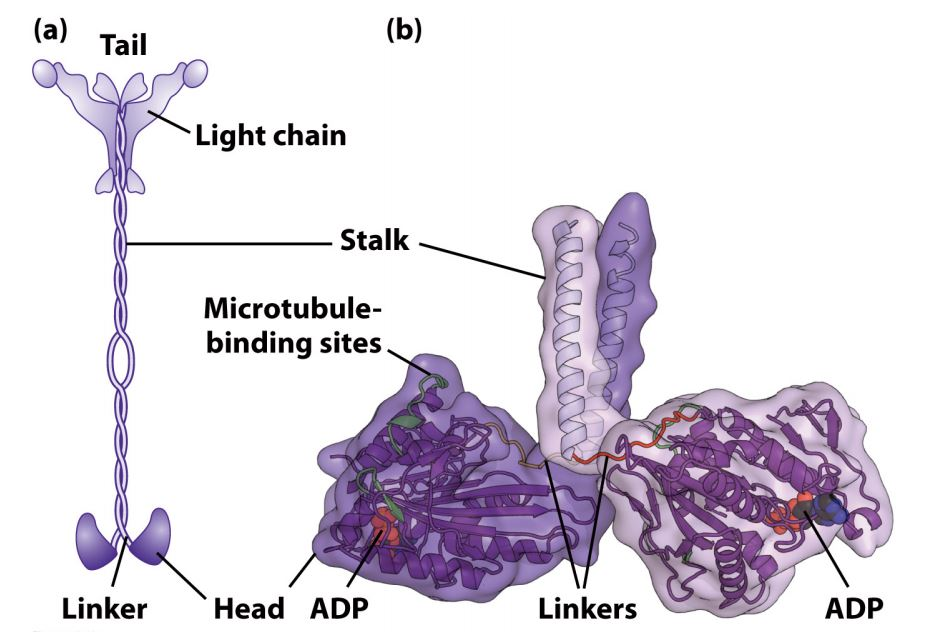
\includegraphics[width=0.5\textwidth]{images/chinesina.JPG}
                    \caption{\small chinesina 1}
                    \label{fig:mesh1}
                \end{figure}
                \begin{itemize}
                    \item Chinesina 1 (CHI1) è un eterodimero, la più classica rappresentata in figura
                    \item Chinesina 2 (CHI2), è un eterotrimero (due catene pesanti diverse che si associano a un terzo polipeptide che determina inetrazione con il cargo).
                    \item Chinesina 5 (CHI5), un tetrametro formato da due coiled coil e quattro piedini. Forma contatti con due MT ed è per questo utilizzato nei processi che necessitano di sliding (entrambe le coppie scorrono nello stesso verso).
                    \item Chinesina 13 (CHI13), è un dimero di cui la quasi totalità è rappresentata dai piedini (non hanno uno stelo). Non è destinato al movimento ma alla catalizzazione della depolimerizzazione dei MT.
                \end{itemize}
                
            \textbf{Movimento}\\
                Il movimento delle CHI è dovuto all'idrolisi di un ATP per ogni "passo" (16 nm, ovvero la distanza tra due dimeri di $\alpha$T e $\beta$T).
                Chiamiamo per chiarezza i due piedini $x$ e $y$. 
                \begin{enumerate}
                    \item Il piede $x$, ora posto davanti (leading head), verso la direzione target, non è legato a nucleotidi: per questo motivo è saldamente legata al MT. $x$ lega un ATP, il quale ingresso induce un irrigidimento che promuove il movimento dei $y$.
                    \item Il piede $y$, posto dietro (trailing head), possiede un ATP che idrolizza ad ADP per allentare il suo legame con MT. Essendo $x$ saldamente legato al MT e quindi svolge la funzione di perno, $y$ arriva in posizione anteriore diventando leading head.
                    \item  $y$ ora si trova ad essere la trailing head e per rafforzare il legame al MT espelle ADP. Quindi il ciclo ricomincia.
                    \item La CHI non si dissocia mai dal MT quindi ha un comportamento processivo.
                \end{enumerate}
                La CHI non si dissocia mai dal MT quindi ha un comportamento processivo.
                \begin{figure}[h]
                    \centering
                    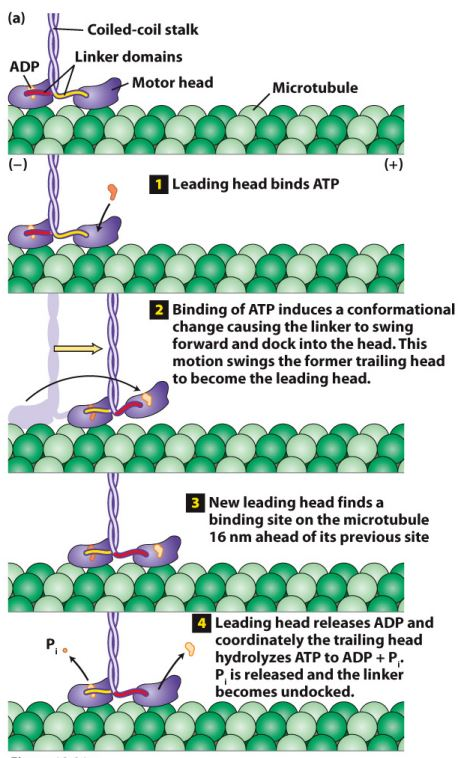
\includegraphics[width=0.5\textwidth]{images/chinesinMovement.JPG}
                    \caption{\small movimento della chinesina}
                    \label{fig:mesh1}
                \end{figure}\\
                
            \textbf{Conformazioni}\\
                Le CHI possono assumere delle conformazioni attive o inattive.\\
                Le conformazioni attive legano in cargo e un MT.
                Le conformazioni inattive sono tali per cui la CHI si ripiega su se stessa. In questo modo si inibisce la funzione catalitica e la proteina viene trasportata da un altro agente all'estremità negativa per poter essere nuovamente utilizzata.
            
        \subsubsection{Dineine}
            Le dineine (DIN) sono proteine di trasporto molto più grandi delle CHI, che solitamente si muovono dall'estrermità positiva a quella negativa (senso retrogrado). \\
            Si differenzia tra DIN citoplasmatica e flagellare.\\
            
            \textbf{Struttura}\\
                Essendo la DIN una molecola molto grande, non è ancora del tutto noto il suo comportamento e la sua struttura.\\
                Sono formate da una catena pesante, una catena leggera e una catena intermedia. La catena pesante è composta da più di 4000 AA (supera i 550 kDalton).\\
                Le DIN hanno delle teste che svolgono attività ATPasica: sono dei conglomerati di sei domini proteici che formano un anello che in termini strutturali è costituito da AAA ATPasi. Il ripiegamento di questo polipeptide fa si che si generino i gambi per protrusione per formare la testa della DIN.\\ 
                Due copie di questo polipeptide formano due "piedini" per camminare sui MT.\\
                Il "cammino" della DIN è dovuto a un cambio conformazione che consiste in un cambio dell'angolo tra lo stelo e l'esamero.\\
                
            \textbf{Interazione con il cargo}\\
                Le DIN interagiscono con un complesso chiamato \textit{dinactina} che concorre a stabilire interazioni con il cargo. La sua subunità \textit{dinamitina} stabilisce l'interazione tra DIN e dinactina. Anche DIN lavora in maniera processiva.
                \begin{figure}[h]
                    \centering
                    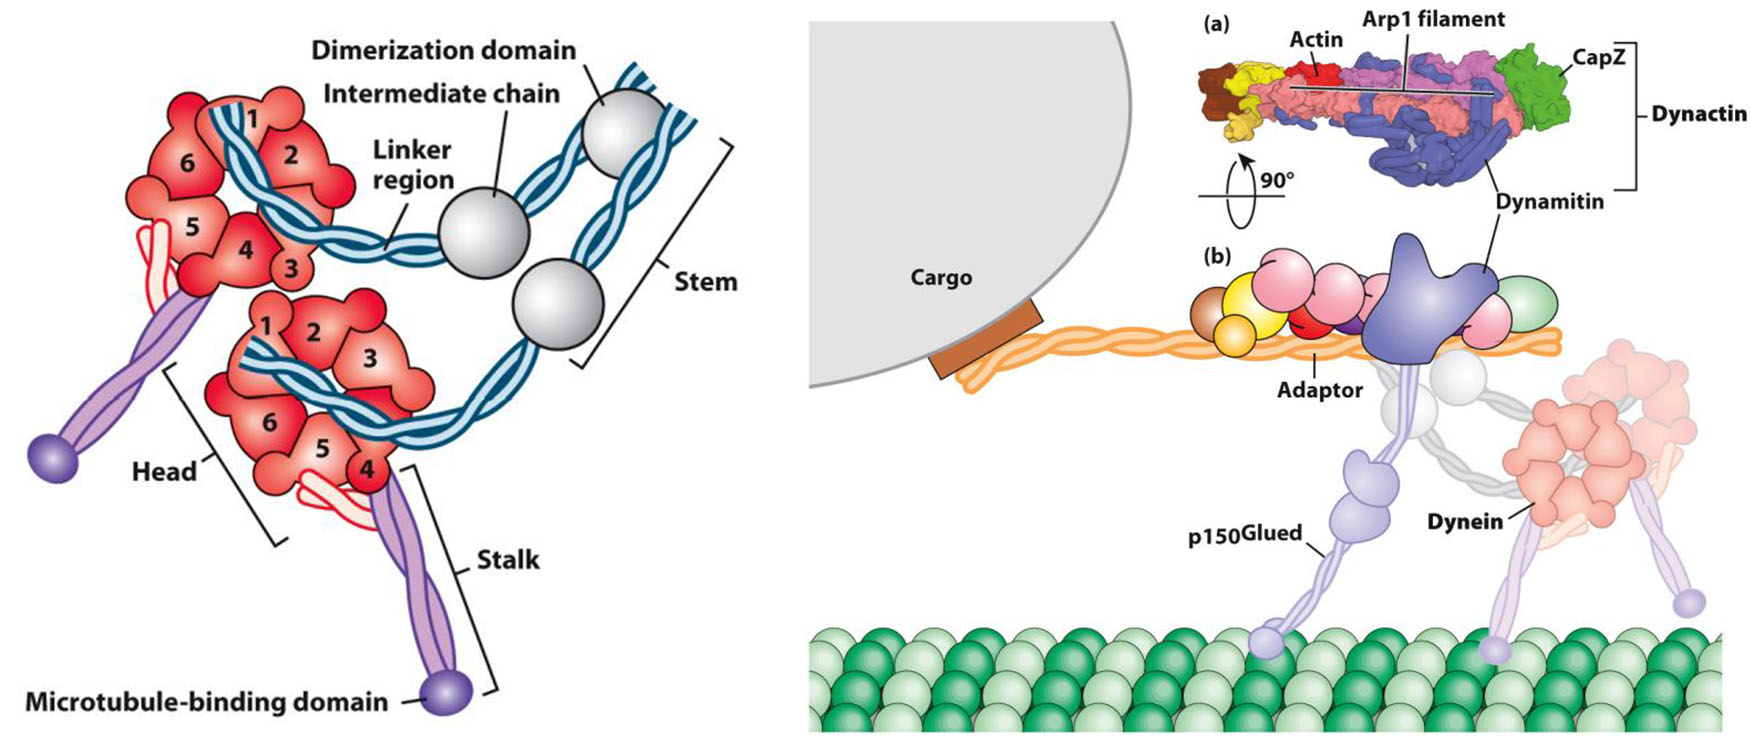
\includegraphics[width=1\textwidth]{images/dineina.JPG}
                    \caption{\small a sinistra struttura della dineina, a destra l'interazione con il cargo}
                    \label{fig:mesh1}
                \end{figure}
                
        \subsection{Interazioni e modifiche}
            Organelli differenti interagiscono con motor proteins diverse. In base a ciò si definiscono strutture e disposizioni differenti interne alla cellula.\\
            I melanofori (cellule dell'epidermide di rettili e pesci), contengono vescicole (melanosomi) con pigmenti che modificano il colore in base alla loro posizione, dettata per l'appunto dal movimento sui MT dei melanosomi.\\
            
            $\alpha$T e $\beta$T possono subire modifiche post-traduzionali. In particolare possiamo assistere a:
            \begin{itemize}
                \item poli glutammilazione sia per $\alpha$T che per $\beta$T che ne promuove la stabilità
                \item poli glicinazione sia per $\alpha$T che per $\beta$T che ne promuove instabilità\\
                Poli glutammilazione è mutualmente esclusivo rispetto a poli glicinazione.
                \item detirosinilizzazione per $\alpha$T che determina la propensione per la CHI13 a depolimerizzare il MT (con questa modifica sono più resistenti alla depolimerizzazione)
                \item acetilazione della lisina per $\alpha$T presenti all'interno della struttura nel caso di cilia o flagelli
            \end{itemize}
            Combinazioni di modifiche determinano comportamenti diversi (CHI1 si associa preferibilmente con MT detirosinati e acetilati).
        
    \subsection{Cilia e flagelli}
        Sono protrusioni costituite in gran parte da MT ricoperte da membrana (e ne richiedono la presenza per resistere). 
        \subsubsection{Struttura}
            Sono costituite da una porzione basale che contiene l'MTOC (un corpo basale, è effettivamente un centriolo) composto da nove triplette e la ruota solitamente presente nel centriolo figlio. Da qui vengono nucleate doppiette di MT. Ha due MT centrali.\\
            C'è una zona di transizione che funge da filtro tra parte interna ed esterna.
            Per assonema si intende la protrusione che può avere lunghezze molto variabili (da micrometri a millimetri). 
            La nessina connette le doppiette di MT, le strutture a raggio conferiscono rigidità, all'interno sono sempre presenti i due MT singoli.
            \begin{figure}[h]
                \centering
                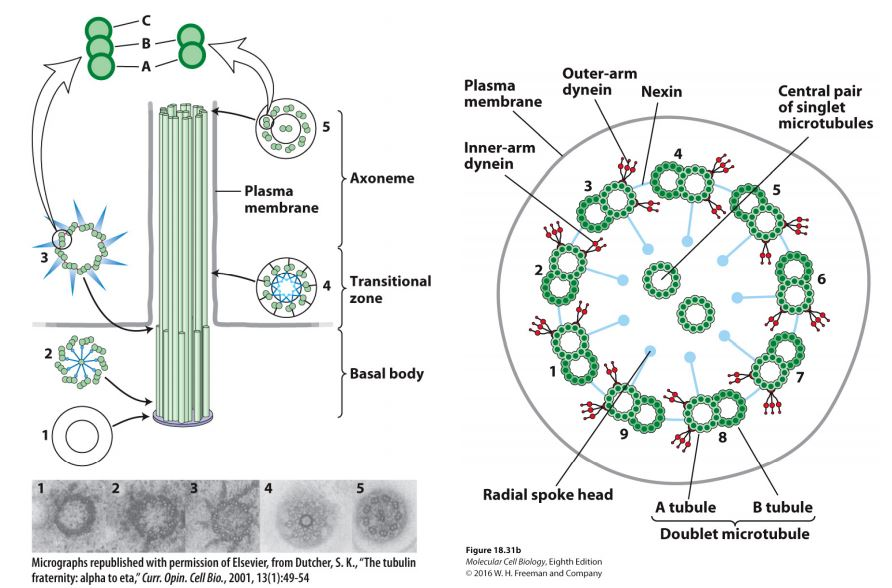
\includegraphics[width=0.6\textwidth]{images/cilia.JPG}
                \caption{\small struttura del cilio o flagello}
                \label{fig:mesh1}
            \end{figure}
        
        \subsubsection{Dineina flagellare}
            I flagelli utilizzano la DIN flagellare, che ha una conformazione differente da quella vista nei paragrafi precedenti. Ha una funzione di movimento del flagelli attraverso attività ATPasica (e non di trasposto).
            Concorre anche al ripiegamento del flagello: la DIN sostiene uno slittamento tra le coppie di MT, la nessina non permette che i due MT scorrano interamente l'uno sull'altro.
            
        \subsubsection{Cilio primario}
            Nel flagello avviene un trasporto attivo di ITF-particles, sostenuto da CHI2 e DIN citoplasmatica, è vitale per la funzione del flagello.
            In moltissime cellule umane/animali esiste il cilio primario che serve come "antenna" per captare segnali provenienti da altre cellule. Ha una struttura differente dal cilio presentato prima, non ha DIN flagellare e non ha i due MT centrali.\\
            La presenza del cilio primario è associata a periodi della vita della cellula in cui è proliferante, viene degradato per permettere al centrosoma di svolgere le funzioni pertinenti alla duplicazione.\\
            Le appendici distali e sub-distali sono necessari per diventare corpuscolo basale, infatti sono necessarie per nucleare i MT del cilio. Difetti nella ciliogenesi causano patologie fenotipicamente e geneticamente molto eterogenee.
    
    \subsection{MT nel ciclo cellulare}
        Il ciclo cellulare si divide in cinque fasi principali: G0, G1, S, G2 e M.\\
        La fase G0 è la fase di vita cellulare non in replicazione. \\
        La fase G1 è la fase in cui viene replicato il materiale cellulare, è presente un solo centrosoma con due centrioli circondati da PCM (peri-cerntiolar material) con $\gamma$T, organizzano MT nello spazio.\\
        La fase S presenta i cromatidi replicati e sono coesi (anello “intrappola” due doppie eliche DNA dei cromatidi fratelli).
        Ogni centriolo genera un pro-centriolo (non maturo), generata da centriolo madre, crescita ortogonale al centriolo madre (mediato da PLK – 4, chinasi).\\
        In fase G2 vi è una doppia quantità DNA, i cromatidi fratelli sono legati da anelli di coesina. Sono presenti 4 centrioli.\\
        La durante la fase M c'è un coinvolgimento più vario dei MT\\	In questa fase avviene la compattazione della cromatina, la trascrizione è sospesa perché dovrà essere separata in due cellule. Ogni centrosoma può liberamente percorrere spazio e formare i due MTOC separati. \\
        Ci sono tre tipi di MT:
        \begin{itemize}
            \item astrali: contatti con cortex e orientamento
            \item polari: interdigitazione, rigidità strutturale
            \item in contatto con cinetocori: contatto con uno dei due cromatidi fratelli
        \end{itemize}
        
        \subsubsection{Profase}
            In profase avvengono i seguenti step:
            \begin{enumerate}
                \item separazione dei due MTOC
                \item riorganizzazione estesa della rete dei MT
                \item condensazione cromosomi
                \item assemblaggio cinetocori
                \item dissoluzione parziale anelli di coesina
            \end{enumerate}
            In particolare la separazione dei centrioli avviene grazie alla CHI-5 che opera lo scorrimento dei MT antiparalleli (allontanamento centrosomi).
            
            L'assemblaggio dei cinetocori (complesso proteico presente sulla porzione centrale del cromosoma in corrispondenza del DNA centromerico) prende luogo perchè possa interagire con i MT. 
            La sua formazione è dovuta a differenza locale nella struttura istonica (CEMP-A al posto di H3, dalla quale dipende la formazione delle altre proteine del cinetocore). Il cinetocore presenta siti per interazione con l’estremità + dei MT.
            
            Infine vengono dissolti gli anelli di coesina ad eccezione che nella zona centromerica (conferendo la tipica forma a X), il quale evento segna la fine della profase.
            \begin{figure}[h]
                \centering
                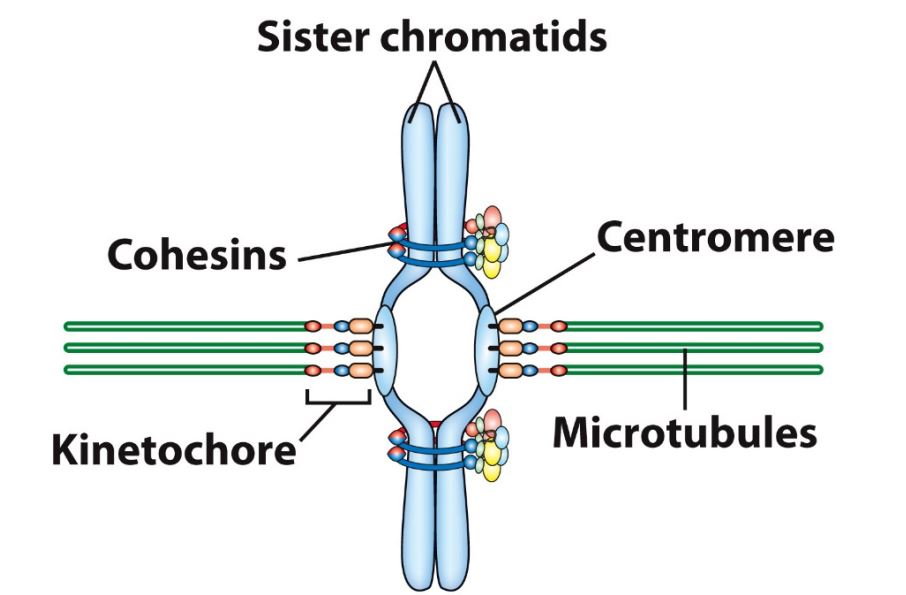
\includegraphics[width=0.5\textwidth]{images/cromatidi.JPG}
                \caption{\small Cromatidi fratelli, cinetocore fornisce ancoraggio a MT}
                \label{fig:mesh1}
            \end{figure}
            
        \subsubsection{Prometafase}
            In prometafase avvengono i seguenti eventi:
            \begin{enumerate}
                \item dissoluzione della membrana nucleare
                \item cattura dei cromosomi da parte dei MT
                \item bi-orientazione e congression
            \end{enumerate}
            Dal momento che cromosomi e MT si trovano nello stesso ambiente (citoplasma) può avvenire l’interazione tra l’estremità + dei MT e il cinetocore.\\
            Di seguito le fasi e le nozioni per sintetizzare bi-orientazione e congression:
            \begin{enumerate}
                \item un cromosoma si dice mono-orientato quando viene agganciato da un MT
                \item si oppongono al movimento netto di un centrosoma mono-orientato verso il centrosoma varie forze (che consistono di molti fattori, es: CHI-4) per arrivare alla bi-orientazione (per congression si intende movimento che prevale)
                \item un cromosoma di dice bi-orientato quando si stabilisce una tensione equilibrata tra i due poli della cellula, quindi quando ogni cromatidio è associato a MT di MTOC diversi
                \item i cromosomi bi-orientati convergono sulla piastra metafasica (anche in tempi diversi)
            \end{enumerate}
            
            \textbf{Regolazione MT e cinetocore con Ndc80 e Aurora B}\\
            \textit{Ndc80 è un complesso (presente in molte copie) la cui formazione innata attorno si MT favorisce l’interazione con il cinetocore. Presenza regolata anche con modifiche post-traduzionali.\\
            Aurora B è una chinesina che fa parte di CPC (Chromosomal Passenger Complex) ed è presente sul centromero. \\
            Si genera una tensione che deforma regioni centrometiche, cinetocore esterno viene orientato verso i poli del fuso per separare i cromatidi promuovendo una defosforilazione di Ncd80 (da parte di Aurora B) e i cinetocori sono più affini ai MT.\\
            L’interazione tra Ncd80 e Aurora B costituisce un metodo per correggere errori (error correction) dovute a tensioni differenti su un cromosoma. Così facendo infatti si destabilizza l’interazione con i MT e la mitosi non può continuare.\\
            \[L'autore non ha capito questa parte\]}
        \subsubsection{Metafase}
            Durante la metafase (definita per esclusione) in cui i cromatidi fratelli sono bi-orientati e sono riusciti a convergere sulla piastra metafasica tenuti in tensione.\\ Avviene l'apertura ultimi anelli di coesina in corrispondenza del centromero.

        \subsubsection{Anafase}
            Durante l'anafase avvengono due eventi in simultaneo: il movimento dei cromatidi verso poli opposti, aumento distanza tra cromatidi (A) e l'aumento distanza interpolare con conseguente elongazione del fuso (B).\\
            La fase A contempla i seguenti step: 
            \begin{enumerate}
                \item depolimerizzazione estremità MT positiva dovuta all’aumento di catastrofi, generazione movimento verso il centrosoma (intervento di CHI-13) grazie all’energia generata dalla depolimerizzazione
                \item depolimerizzazione estremità MT negativa, fenomeno di treadmilling CHI13
            \end{enumerate}
            La fase B sono coinvolte CHI-5 che promuovono lo shift dei MT in posizione centrale (antiparalleli) e una DIN associata a MT corticali avvicina il fuso verso la membrana plasmatica.

        \subsubsection{Telofase}
            Avviene la riformazione involucro nucleare.
            
            \begin{figure}[h]
                \centering
                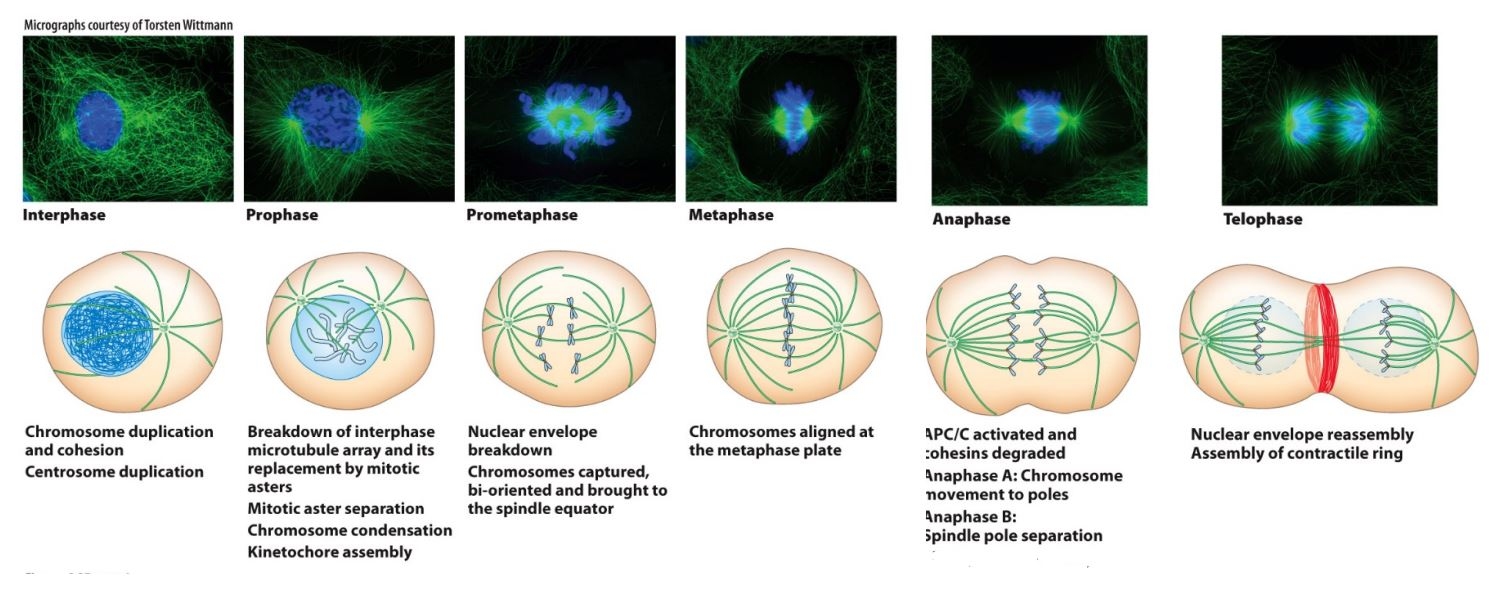
\includegraphics[width=1\textwidth]{images/mitosi.JPG}
                \caption{\small fasi della mitosi}
                \label{fig:mesh1}
            \end{figure}
            
        \subsubsection{Citocinesi e cariochinesi}
            Per citochinesi si intende la separazione fisica a livello citoplasmatico delle due cellule. Non è un processo separato da altre fasi cellulari, ma avviene in simultaneo alle ultime fasi della mitosi, comincia in corrispondenza dell’anafase.\\
            Per cariochinesi si intende la separazione dei nuclei (e corredi genetici), corrispondenti alle prime 5 fasi della meiosi.\\
            
            \textbf{Aurora B e CPC}\\
            In pro/prometa/metafase, Aurora B e CPC sono localizzati al centromero.\\
            Durante anafase si rilocalizzano sulla spindle midzone, hanno affinità con MT antiparalleli e mantengono questa localizzazione anche in telofase.\\
            Si forma un anello contrattile che determina invaginazione (fatto di actina e miosina), che si genera in corrispondenza della posizione di Aurora B (fornisce alla cellula le “coordinate” per la separazione).
            
\section{Filamenti intermedi}
    I FI hanno una composizione eterogenea tessuto-specifica. Hanno un diametro di circa 10 nm.
    Sono presenti anche all'interno del nucleo. Danno rigidità ai tessuti, non hanno polarità intrinseca, non sono legate a nucleotidi fosfati, non sono note proteine motore che interagiscono con FI (correlato al fatto che non hanno polarità) e hanno dinamicità limitata.
    
    \subsection{Struttura}
        70 geni differenti codificano per i FI. Sono dei dimeri paralleli che formano dei coiled coil. I domini C e N terminali sono specifici in base al tessuto e possono essere tra loro molto diversificati. Ogni dimero può associarsi ad un altro dimero in modo antiparallelo.\\
        Un protofilamento è composto da 4 FI associati in maniera antiparallela, 4 protofilamenti formano una \textit{protofibrilla}.
        \begin{figure}[h]
            \centering
            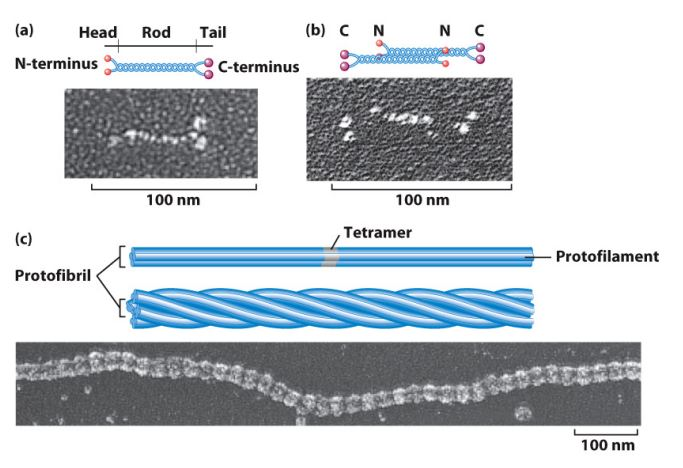
\includegraphics[width=0.7\textwidth]{images/filametiIntermedi.JPG}
            \caption{\small struttura dei FI e della protofibrilla}
            \label{fig:mesh1}
        \end{figure}
    \subsection{Classi}
        I FI si dividono in classi.
        \subsubsection{Cheratina acida e basica}
            Sono due classi differenti (acida e basica) che però collaborano strettamente, sono sempre associate a coppie acida-basica. Sono codificate da 50/70 geni e sono ampiamente presenti a livello epiteliale. Contribuiscono alla rigidità della cellula.
        \subsubsection{Desmina, vimentina e GFAP}
            Sono FI presenti delle cellule muscolari, gliali e mesenchimali. Si occupano dell'organizzazione del sarcomero e hanno funzioni tra loro differenti.
        \subsubsection{Neurofilamenti}
            Sono presenti nelle cellule neuronali e contribuiscono all'organizzazione dell'assone. Si dividono in categorie differenti perchè sono tre tipologie che collaborano (light, heavy e medium).
        \subsubsection{Lamìne}
            Sono FI presenti nel nucleo che contribuiscono alla sua organizzazione e struttura.
            Sono ubiquitari, in assoluto i più comuni. Interagiscono con il cortex per la membrana nucleare. \\
            Le lamìne formano un reticolo sottostante alla membrana nucleare (interna) e si associa alla membrana in modi differenti (tramite proteine o la sua struttura è modificata direttamente per l'interazione). \\
            Interagisce con la cromatina per il suo metabolismo, preferibilmente con regioni eterocromatiche.\\
            La mutazione di questa proteina compromette la stabilità del DNA.\\
            Risulta in continuità con altri elementi citocheletrici citoplasmatici, infatti esistono proteine specifiche che consentono l'interazione della lamìna con MT, FI e MF.\\
            Esistono proteine diverse che sostituiscono la classe delle lamìne [A, B1, B2, C]. Le proteine A e C derivano dallo splicing alternativo dello stesso gene.\\
            In prometafase, la dissoluzione del nucleo avviene anche grazie alla fosforilazione della lamìna (che è un processo reversibile).

\section{Microfilamenti}
    I microfilamenti (detti anche filamenti di actina) sono intimamente legati alla membrana citoplasmatica, sono deputati al movimento della cellula e alla definizione della forma della membrana. In cellule polarizzate definisce il leading edge. I MF determinano la forma della cellula in base ai segnali dei recettori delle membrane: l'actina è la componente citoschelettrica più fortemente condizionata dal signaling. Hanno un diametro di 6/7 nm.\\
    L'actina ha strutture e funzioni diverse:
        \begin{itemize}
            \item microvilli
            \item cortex cellulare
            \item connessione cellule
            \item movimento delle vescicole
            \item formazione lamellipodi e fillopodi
            \item stress fibers (presenti fisiologicamente)
            \item fagocitosi
            \item anello contrattile
        \end{itemize}
    A livello sperimentale viene utilizzata la \textit{falloidina} che lega l'actina e ne permette l'osservazione "immobilizzandola" nel caso di cellule vive.
    
    \subsection{Struttura}
        L'actina è composta da un singolo polipeptide ed è codificata da molteplici geni. Il singolo monomero che compone il filamento di actina (F-ACT) è l'actina globulare (G-ACT) che presenta una tasca per l'associazione con l'ATP.\\
        Il F-ACT è polarizzato (l'estremità positiva non espone la tasca per ATP, quella negativa si), sono necessarie 14 G-ACT per compiere un giro.\\
        La miosina è una proteina che interagisce fortemente con l'actina e che si lega ad essa con un angolo specifico, osservando l'angolo si deduce l'orientamento del F-ACT (si forma una "freccia" che indica l'estremità negativa).
        \begin{figure}[h]
            \centering
            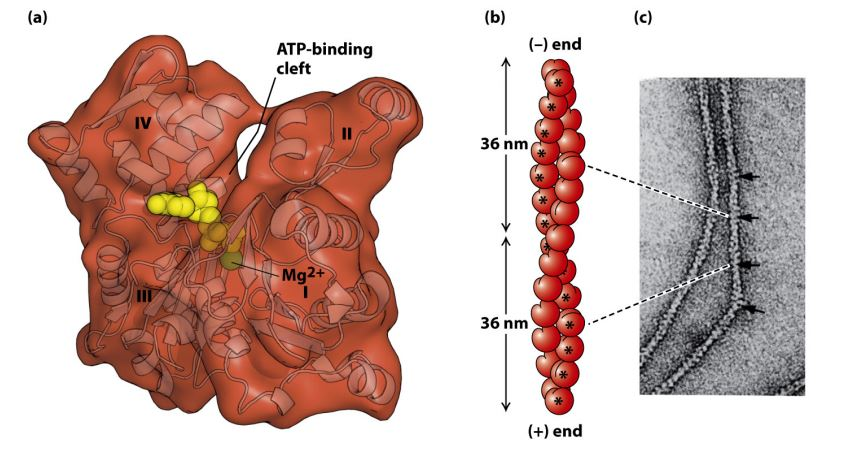
\includegraphics[width=0.7\textwidth]{images/G-ACTeF-ACT.JPG}
            \caption{\small Struttura della actina globulare e del filamento}
            \label{fig:mesh1}
        \end{figure}
        
        \subsubsection{Comportamento dell'actina purificata}
            In vitro si riesce a studiare il comportamento dell'actina purificata per quanto riguarda la sua crescita e decrescita. Si notano tre fasi: lag, elongation e una fase di stallo.
            \begin{enumerate}
                \item LAG: è la fase iniziale a cui si assiste alla formazione di un nucleo di tre G-ACT che costituiscono il seme su cui si baserà l'orientamento e la struttura di tutto il F-ACT.
                \item ELONGATION: una fase di rapida elongazione del filamento
                \item STALLO: equilibrio tra concentrazione di G-ACT e quella presente su F-ACT. Avviene in corrispondenza della concentrazione critica CC.
            \end{enumerate}
            
    \subsection{Dinamica dei MF}
        La dissociazione della G-ACT avviene a prescindere dalla sua concentrazione. L'aggiunta a un F-ACT di G-ACT dipende invece dalla concentrazione, la concentrazione critica dell'estremità positiva differisce da quella all'estremità negativa.
        La G-ACT possiede un'innata propensione ad idrolizzare ATP e rilasciare il fosfato. All'equilibrio il dominio positivo di F-ACT possiede ATP, i domini intermedi ADP+P e quella negativo solo ADP.\\
        L'idrolisi dell'ATP riduce la propensione della G-ACT a rimanere associata a un F-ACT.
        Anche i MF presentano il processo di treadmilling (l'accrescimento all'estremità positiva, depolimerizzazione all'estremità negativa).
        Il treadmilling del preparato di sola actina è è 10 volte pià rapido di quello espresso in vivo.
            
        \subsubsection{Agenti promotori ed inibitori}
            Ci sono degli agenti che ne modificano il comportamento:
            \begin{itemize}
                \item Profilina: lega G-ACT legata a ADP e catalizza lo scambio con ATP, quindi ne velocizza la polimerizzazione.
                \item Cofilina: lega protofilamenti di F-ACT e ADP e ne catalizza la depolimerizzazione all'estremità negativa.
                \item Timosina $\beta$4: lega G-ACT e ATP quando questa è monomerica. In questo modo non può essere incorporata in un F-ACT (si forma una "riserva").
                \item CapZ e Gelsoina: si legano all'estremità positiva e previene l'aggiunta di F-ACT. Promuove la decrescita.
                \item Tropomodulina: si lega all'estremità negativa di F-ACT e ne previene il disassemblaggio. Promuove la crescita.
                \item Formina: è una proteina composta di più domini catalizza l'assemblaggio di F-ACT. Il dominio FH2 stabilisce il contato tra due G-ACT orientate correttamente e possibilmente cambia conformazione man mano che si aggiunge G-ACT. Il dominio FH1 ha affinità per profilina che promuove una crescita locale. Il dominio RBD interagisce con $\rho$GTP, regola il ripiegamento per l'autoinibizione (in assenza di $\rho$GTP) o scatena l'attività della formina in sua presenza.
                Può inibire l'associazione con CapZ rimanendo associata all'estremità positiva.
                \item Complesso ARP (\textit{actin related protein}): consiste di sette subunità, promuove la nucleazione di G-ACT con ramificazione. Utilizza NPF (\textit{nucleation promoting factor}) che predispone la G-ACT spazialmente per la nuova nucleazione di F-ACT. Il ramo cresce inclinato di 70° e sono strutture ricorrenti nei lamellipodi.
                Alcune NPF (per esempio WASp) vengono mantenute inattive finchè non intervengono due segnali contemporaneamente scatenati da input diversi. \\
                L'actina ramificata contribuisce anche alla fagocitosi. Un leucocita incapsula un battere riconosciuto tramite un anticorpo, promossa dalla locale attivazione di ARP 2/3.
                \end{itemize}
                \begin{figure}[h]
                    \centering
                    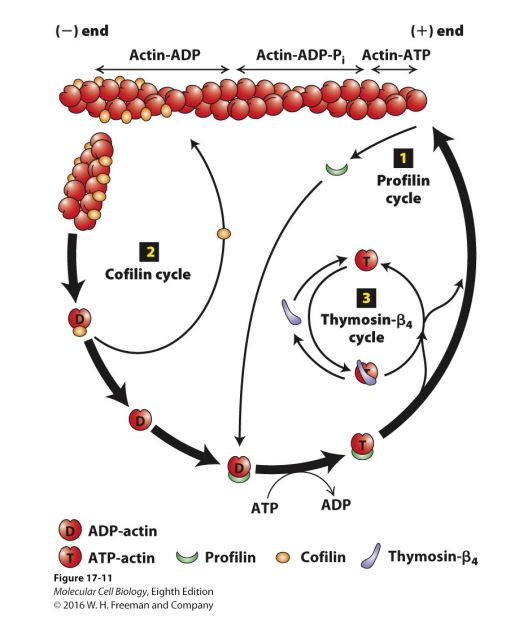
\includegraphics[width=0.7\textwidth]{images/agentiActina.JPG}
                    \caption{\small interazione timosina, profilina e cofilina con il filamento di actina}
                    \label{fig:mesh1}
                \end{figure}
            
        \subsubsection{Strutture particolari con fattori di movimenti}
            Si possono formare strutture di MF più complesse con l'interazione di ACLP (\textit{actine cross linking proteins}) che hanno più siti di legame per l'organizzazione dei filamenti nello spazio. Ricordiamo tra queste $\alpha$actina, fimbrina, spectrina, filamina e distrofina.   \\
            La spectrina è una molecola che organizza i MF in prossimità del cortex con una disposizione a raggera. Funge anche da hub tra proteine di membrana.\\
            La distrofina può essere geneticamente difettosa, in quel caso può causare patologie quali la distrofia muscolare (ma non solo).
            
    \subsection{Miosine}
        Le miosine, sono una famiglia di proteine che funge da motor protein per i MF. Hanno in comune una testa ma la coda è specifica. Il loro movimento deriva dall'idrolisi dell'ATP e assumono molti aspetti specifici (sono codificate da circa 40 geni diversi). Esistono molteplici mutazioni di questi 40 geni che causano patologie anche ereditarie.\\
        In generale camminano verso l'estremità positiva (tranne la miosina 6).
        
        \subsubsection{Miosina 1}
            La MI1 ha a caratteristica di avere una sola catena pesante, il suo passo corrisponde a 10-14 nm, è associata alla membrana e sostiene l'endocitosi. Alcuni membri di MI1 interagiscono direttamente con i lipidi.
            
        \subsubsection{Miosina 5}
            La MI5 ha una \textit{duty rate} di circa il 70\% quindi risulta molto processiva ed è coinvolta nel trasporto di organelli. La porzione della proteina che si pone tra lo stelo e i piedi è più allungata e quindi ha un passo di lunghezza maggiore (passo di 36 nm).\\
            La MI5 è utilizzata nella duplicazione del lievito (\textit{budding yeast}), si forma infatti un F-ACT nella nuova gemma e MI5 trasporta diverse molecole e organelli in direzione della gemma (anche estremità di MT).\\
            Anche nell'uomo è presente la MI5 ma se sue funzioni non sono ben comprese e definite come per il lievito.
            
        \subsubsection{Miosina 6}
            La MI6 è eccezionalmente una miosina che cammina vero l'estremità negativa del filamento di actina.
            
        \subsubsection{Miosina 2}
            La miosina 2 (MI2) è quella storicamente più importante, è ampiamente presente nel muscolo scheletrico e anche nelle cellule muscolari cardiache. Ne esistono circa 20 tipi diversi.    \\
            Esistono 16 geni che le codificano, utilizzano ATP per il lavoro meccanico e sono presenti anche in tessuti non muscolari. Il loro passo compie 8 nm.\\
            
            \textbf{Struttura}\\
            Sono composte da una catena pesante formata da un coiled coil, delle catene leggere regolatrici e leggere essenziali e dei siti attivi. Le ultime tre componenti insieme (porzione S1) lega direttamente l'actina e il nucleotide tri-fosfato. Migra verso il polo positivo dell'actina.\\
            \begin{figure}[h]
                \centering
                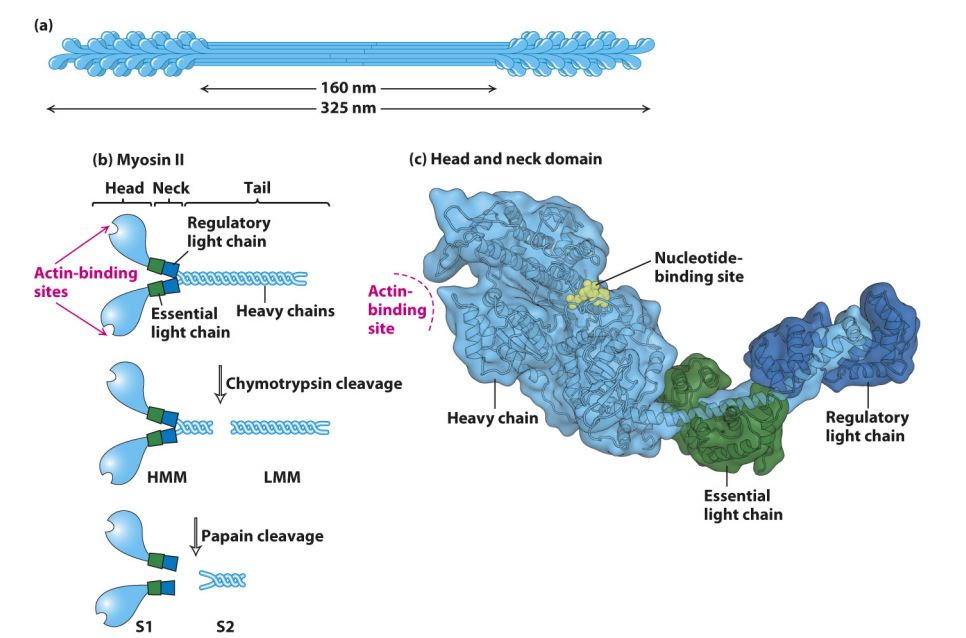
\includegraphics[width=0.7\textwidth]{images/miosina.JPG}
                \caption{\small Struttura della miosina2}
                \label{fig:mesh1}
            \end{figure}
            
            \textbf{Cammino}\\
                Il movimento della MI2 è possibile grazie all'idrolisi di ATP e il suo passo è di 8nm. 
                In particolare avviene secondo questi step:
                \begin{enumerate}
                    \item legame al MF saldo, MI2 non è legata ad ATP
                    \item rilascio della testa e legame con ATP
                    \item idrolisi dell'ATP causa un movimento del dominio
                    \item nuovo contatto con MF e rilascio dell'ADP per saldarsi all'actina
                \end{enumerate}
                Alterando la lunghezza del collo della MI si ottiene una velocità differente (proporzionale all'allungamento del passo). \\
                Per \textit{duty rate} si intende la percentuale di tempo che la testa passa legata al MF. Questo periodo dipende dalla propensione a rilasciare ADP. La duty rate di MI5 è maggiore di MI2. \\
            
            \textbf{Regolazione contrazione}\\
                Le cellule muscolari si assemblano in strutture superiori chiamate \textit{sincizi}. Queste consistono in cellule plurinucleate e si organizzano in fasci. I sincizi vano a loro volta a formare le miofibrille, la cui contrazione è regolata dal sarcomero: un assemblamento di ACT e MI. \\
                Nel sarcomero sono presenti anche altri agenti, in parte già visti in precedenza, quali:
                \begin{itemize}
                    \item titina: in continuità tra ACT e MI
                    \item nebulina: determina la lunghezza dell'ACT
                    \item tropomodulina, troponina e tropomiosina
                    \item CapZ
                \end{itemize}
                La contrazione viene regolata in dipendenza da ioni calcio $Ca^{++}$.
                \begin{enumerate}
                    \item arriva un segnale nervoso che rilascia ioni $Ca^{++}$ dal reticolo sarcoplasmatico. 
                    \item aumento della concentrazione di $Ca^{++}$ citoplasmatica
                    \item $Ca^{++}$ lega una subunità della troponina (a sua volta legata alla tropomiosina) associata ai F-ACT
                    \item spostamento della tropomiosina, esposizione dei siti di legame con la MI prima mascherati
                    \item contatto MI2 e F-ACT che determinano la possibilità di entrare nel ciclo di contrazione
                \end{enumerate}
                \begin{figure}[h]
                    \centering 
                    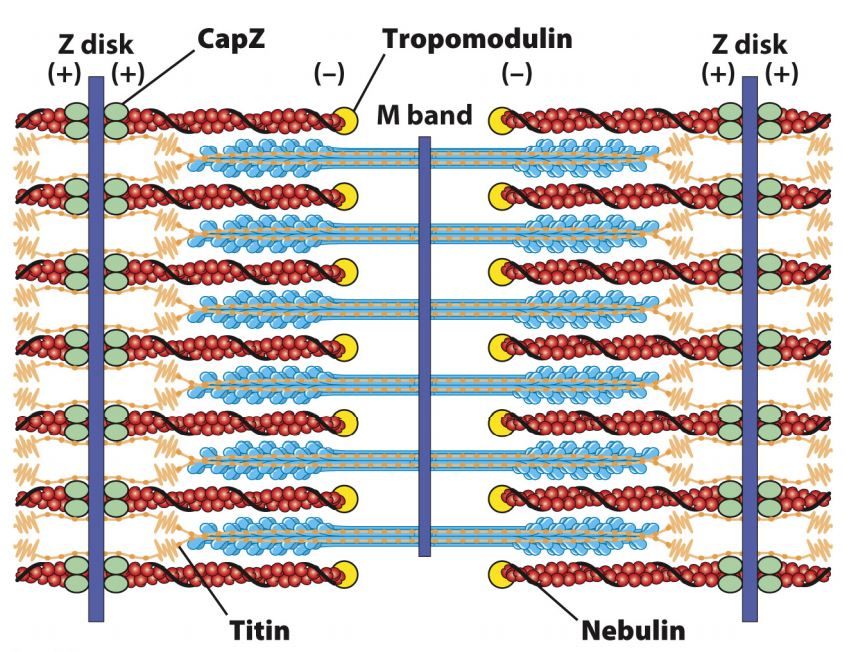
\includegraphics[width=0.5\textwidth]{images/sarcomero.JPG}
                    \caption{\small Struttura del sarcomero}
                    \label{fig:mesh1}
                \end{figure}
            
            \textbf{Contrazione nel tessuto muscolare liscio}\\
                Il tessuto muscolare liscio non presenta sarcomeri, la sua contrazione avviene senza l'interazione tra ACT e MI.
                La contrazione avviene per un meccanismo di fosforilazione e defosforilazione di una proteina target, ovvero la catena leggera regolatoria.\\
                ATP cede il suo P alla proteina target che forma un legame covalente. Il bilancio energetico è favorevole. Questo evento cambia la conformazione della proteina target che ne modifica l'attività.
                A seconda della proteina target, può essere la defosforilazione che determina il suo attivamento.\\
                \textbf{Gli AA che tipicamente possono essere fosforilati sono serina, treonina e tirosina}. La fosforilazione viene tipicamente promossa da una protein-chinasi per serina e treonina o tirosina (due gruppi di protein-chinasi) o da una protein-fosfatasi.\\
                La MI2 può essere regolata dalla fosforilazione della catena leggera che quindi regola l'esposizione del Coiled coil e la contrazione. Protein chinasi e fosfatasi collaborano per la contrazione. In particolare avvengono questi step:
                \begin{enumerate}
                    \item $Ca^{++}$ provoca un segnale
                    \item $Ca^{++}$ lega la CAM (calmodulina) e attiva MLC-chinasi
                    \item contrazione
                \end{enumerate}
                Il meccanismo regolato in questo modo risulta molto più lento perchè $Ca{++}$ deve diffondere nella cellula senza sarcoplasma.\\
                
            \textbf{Altre funzioni di MI2}\\
                La MI2 è impiegata anche per la formazione dell'anello contrattile (assieme all'ACT) durante anafase e telofase per la citochinesi. \\
                Assieme all'ACT, MI2 ha un ruolo fondamentale per la formazione di anelli contrattili a livello apicale delle cellule epiteliali.\\
                
            \textbf{Tossine}\\
                Esistono varie tossine che alterano il comportamento della MI2, quali:
                \begin{enumerate}
                    \item citocalesina B e D, che impedisce la polimerizzazione di ACT legandosi all'estremità positiva
                    \item latrunculin che impedisce la polimerizzazione legando la G-ACT
                    \item falloidina che previene la depolimerizzazione, quindi ne impedisce la dinamicità
                \end{enumerate}
            
    \subsection{Migrazione cellulare}
        La coordinazione tra ACT e MI, assieme al livello di concentrazione di $\rho$GTPasi determina gli eventi di locomozione della cellula. Distinguiamo le seguenti strutture e attività della cellula:
        \begin{itemize}
            \item lamellipodio: è l'estensione dell'estremità frontale sostenuta dal treadmilling di ACT ed è regolato da ARP2-3, formazione di ramificazioni di ACT
            \item adesione alla matrice extracellulare ad opera di strutture di adesione focale (mediate da integrine,\textit{ focal adesion}), consente contatto tra citoscheletro interno e matrice extracellulare
            \item traslocazione: lavoro di contrazione di ACT su MI2 interni alla cellula sull'estremità opposto del "senso di marcia"
            \item endocitosi: fase di de-adesione, la nuova membrana che viene utilizzata al leading edge deve essere rigenerata, quindi avviene un riciclo di lipidi di membrana distanti
        \end{itemize}
        
        A livello molecolare, le focal adesion interagiscono con proteine trans-membrana (integrine) che hanno funzioni meccaniche e di signaling per il citoscheletro (oltre che essere ancoraggio fisico). \\
        Le stress fibers sono formazioni di fibre contrattili ACT e MI2 che richiamano l'estremità arretrata.
        
        \subsubsection{Regolazione da cascate di trasduzione del segnale}
            La locomozione cellulare è un esempio di come una cascata di trasduzione di segnali anche extracellulari possano concorrere alla modifica conformazionale della cellula.\\
            La cascata di signaling è operata dalla famiglia di proteine $\rho$, sono GTPasi globulari con ancora lipidica associata alla membrana (foglietto citosolico), possono associarsi a GTP o GDP e in base a questi generano segnale (con GTP interagiscono con proteine effettrici che veicolano segnali a valle). Associata al GDP abbiamo la conformazione inattiva.\\
            Quando $\rho$ è esposta nella membrana interagisce con
            \begin{itemize}
                \item GEF (promozione scambio GDP con GTP) che ne induce attivazione
                \item GAP (promozione idrolisi GTP) che ripristina uno stato inattivo.
            \end{itemize}
            \begin{figure}[h]
                \centering
                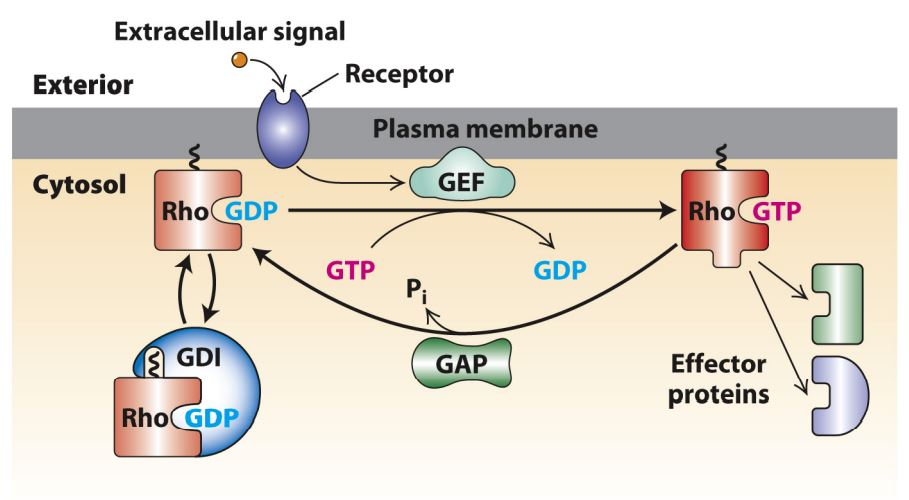
\includegraphics[width=0.5\textwidth]{images/RhoGEFeGAP.JPG}
                \caption{\small Interazione di $\rho$ con GEF e GAP}
                \label{fig:mesh1}
            \end{figure}
            
            \textit{
                \textbf{Dominanza negativa}\\
                Per dominanza negativa si intende una mutazione che influenza negativamente di un gene wild type (wt), può essere una versione di un gene mutata che compromette il corretto funzionamento possibilmente anche di altri complessi. Per le $\rho$GTPasi potrebbe essere una proteina che modifica interazione con GEF.\\}
            
            \textit{    
                \textbf{Dominanza positiva} \\
                Per dominanza positiva si intende un gene mutante che impedisce l'inattivazione di altri complessi. Nel caso delle $\rho$GTPasi, la modifica di un singolo AA muta il legame costitutivo con GTP per esprimere segnali.}\\
            
            Se esprimo nella stessa cellula diversi dominanti attivi di tre diverse $\rho$GTPasi osservo in ogni caso un rimodellamento del citoscheletro di ACT (ognuna singolarmente):
            \begin{itemize}
                \item $\rho$ dominant active determina formazione eccessiva di stress fibers
                \item CDC dominant active determina fillopodi in ogni direzione
                \item RAC dominant active determina la formazione di membrane ruffles
            \end{itemize}
            Un approccio readout molto comune è lo \textit{scretch essay} in cui cresco delle cellule sulla petri, esercito una discontinuità e dopo una certa quantità di tempo le cellule migrano e tornano ad occupare lo spazio dello scatch. 
            I tre dominanti positivi sopra rallentano il processo migratorio di questo esperimento. \\
            Al leading edge, il treadmilling è iniziato e promosso da attivazione di CDC42 (selettivamente alle porzione di membrana frontale al movimento) che determina l'attivazione di RAC (al leading edge) che che interagisce con ARP23 che causa il treadmilling. Al contempo, RAC determina l'attivazione di $\rho$ nella porzione distante della cellula che induce la contrazione dei filamenti di ACT-MI.
            L'interazione inibitoria tra $\rho$ e RAC è importante per compartimentalizzare i comportamenti in porzioni differenti della cellula. Entrambi i processi sono iniziati da CDC42.

\pagebreak